% document type
\documentclass[12pt]{article}
\RequirePackage{pdf14}
\usepackage[total={170mm,230mm}]{geometry}
%Russian-specific packages
%--------------------------------------
\usepackage[T2A]{fontenc}
\usepackage[utf8]{inputenc}
\usepackage[russian]{babel}
%--------------------------------------
 
%Hyphenation rules
%--------------------------------------
\usepackage{hyphenat}

\usepackage{graphicx}
\usepackage{amssymb}
\usepackage{amsfonts}
\usepackage{amsmath}
\usepackage{amsthm}
\usepackage{physics}

\usepackage{hyperref}
\usepackage{cmap}

\newcommand*{\figref}[2][]{\hyperref[#2]{Рис.~\ref*{#2}#1}}
\newcommand*{\tabref}[2][]{\hyperref[#2]{Табл.~\ref*{#2}#1}}
% \newcommand*{\tblref}[1]{\hyperref[#1]{Table~\ref*{#1}}}
\newcommand*{\secref}[1]{\hyperref[#1]{Section~\ref*{#1}}}
% \newcommand*{\secsref}[1]{\hyperref[#1]{Sections~\ref*{#1}}}
% \newcommand*{\introref}[1]{\hyperref[#1]{Introduction}}

\begin{document}
	\input{titlepage}
	\setcounter{page}{2}

	\tableofcontents
	\newpage

	\section{Основные элементы теории}

	\section{Схема установки}

	\begin{figure}[tb]
		\centering
		\includegraphics[width=\textwidth]{../figures/scheme.png}
		\caption{Схема установки.}
		\label{fig:scheme}
	\end{figure}

	Схема экспериментальной установки представлена на \figref{fig:scheme}. В качестве источника накачки используется полупроводниковый лазер (2) со следующими характеристиками
	\begin{enumerate}
		\item длина волны генерации $810\,\text{нм}$;
		\item пороговый ток питания $200\,\text{мА}$;
		\item максимальная мощность излучения $0.5\,\text{Вт}$;
		\item поляризация излучения линейная, вектор электрического поля лежит в вертикальной плоскости.
	\end{enumerate}

	Короткофокусная линза (3) используется для формирования параллельного пучка из сильно расходящегося у торца лазера излучения накачки. Линза (4) закреплена в поворотном устройстве, позволяющем перемещать луч накачки в горизонтальной и вертикальной плоскостях. Резонатор твердотельного лазера (5--7) установлен на платформе, передвигающейся в продольном и поперечном направлениях. В качестве активной среды лазера используется кристалл алюмоиттриевого граната YAG, легированный ионами $\mathrm{Nd}^{3+}$ с концентрацией 1\%. Кристалл Nd:YAG (6) имеет форму цилиндра длинной $1\,\text{см}$ и диаметром $0.6\,\text{см}$. Он закреплён в юстировочном устройстве, позволяющем плавно изменять положение оси кристалла относительно оси резонатора. Торцы кристалла имеют дихроичное покрытие. Один формирует входное зеркало резонатора (5), обеспечивая пропускание света $T\approx 1$ на длине волны $\lambda=810\,\text{нм}$ и отражение $R_1 \approx 1$ на длине волны $\lambda=1064\,\text{нм}$, другой просветлен на длине волны $\lambda=1064\,\text{нм}$. Выходное зеркало резонатора (7), имеющее коэффициент отражения $R_2=0.98\ldots0.995$ на длине волны $\lambda=1064\,\text{нм}$, закреплено в юстировочном устройстве, позволяющем плавно поворачивать его относительно входного зеркала резонатора. Установка позволяет менять длину резонатора от 5 до 7.5 см. Для отсекания излучения накачки на выходе резонатора используется фильтр (8). Излучение Nd:YAG лазера подается через поворотное зеркало (9) на фотодиод (10), выход которого подключен к микроамперметру (12) и анализатору спектра СК4-58 (11). Последний предназначен для наблюдения низкочастотных шумов лазера в диапазоне $0\ldots600$ кГц. He-Ne лазер (15) используется для юстировки резонатора. Для визуального наблюдения генерации Nd:YAG лазера используется карточка-визуализатор инфракрасного диапазона.

	\section{Протокол измерений}

	Измерили зависимость релаксационной частоты $f_\text{рел}$ и мощности излучения $P_\text{изл}$ от мощности накачки $P_\text{нак}$. Результаты измерений приведены в \tabref{tab}.

	\begin{table}[tb]
	\begin{center}
	 	\begin{tabular}{|c|c|}
	 		\hline
	 		$P_\text{нак}$, мВт & $f_\text{рел}$, кГц\\
	 		\hline
			216 &	112\\
			225 &	212\\
			235 &	276\\
			245 &	336\\
			255 &	392\\
			265 &	432\\
			270 &	448\\
			275 &	458\\
			280 &	476\\
			285 &	491\\
			296 &	508\\
			304 &	532\\
			345 &	551\\
			385 &	600\\
			390 &	616\\
			395 &	627\\
			405 &	639\\
			420 &	672\\
			\hline
	 	\end{tabular}
	 	\begin{tabular}{|c|c|}
	 		\hline
	 		$P_\text{нак}$, мВт & $P_\text{изл}$, мВт\\
	 		\hline
	 		420 &	9\\
			410 &	8.37\\
			400 &	7.85\\
			391 &	7.6\\
			381 &	7.3\\
			371 &	6.8\\
			361 &	6.1\\
			350 &	5.5\\
			340 &	4.6\\
			330 &	4\\
			320 &	3.76\\
			290 &	3.3\\
			280 &	2.9\\
			270 &	2.5\\
			260 &	2.1\\
			250 &	1.7\\
			239 &	1.2\\
			230 &	0.9\\
			220 &	0.5\\
			210 &	0.19\\
			200 &	0.14\\
			\hline
	 	\end{tabular}
	\end{center}
	\caption{Результаты измерений.}
	\label{tab}
	\end{table}

	\section{Результаты эксперимента с оценкой погрешности и их сравнение с теорией}

	\subsection{Определение пороговой мощности}

	Для дальнейшей работы важно определить пороговую мощность $P_\text{пор}$, ведь ниже будет часто использоваться параметр накачки $A$, который определяется как $P_\text{нак} / P_\text{пор}$ ($P_\text{нак}$ измеряется напрямую). Чтобы определить пороговую мощность $P_\text{пор}$, надо найти такую мощность накачки, что при мощностях накачки меньше данной мощность излучения равна нулю, а при больших мощностях накачки мощность излучения отлична от нуля.

	На \figref{fig:p_iz_vs_p_nak} показана снятая зависимость мощности излучения от мощности накачки с учётом фоновой засветки. Видно, что при $P_\text{нак}<210\,\text{мВт}$ излучения нет. Снятые данные дискретны и поэтому точно определить порог нам не удастся, мы лишь знаем, что при $P_\text{нак}=210\pm5\,\text{мВт}$ излучение есть, а при $P_\text{нак}=205\pm5\,\text{мВт}$ излучения нет. Порог находится где-то между $200\,\text{мВт}$ и $210\,\text{мВт}$. Значит, $P_\text{пор} = 205\pm5\,\text{мВт}.$

	\begin{figure}[tb]
		\centering
		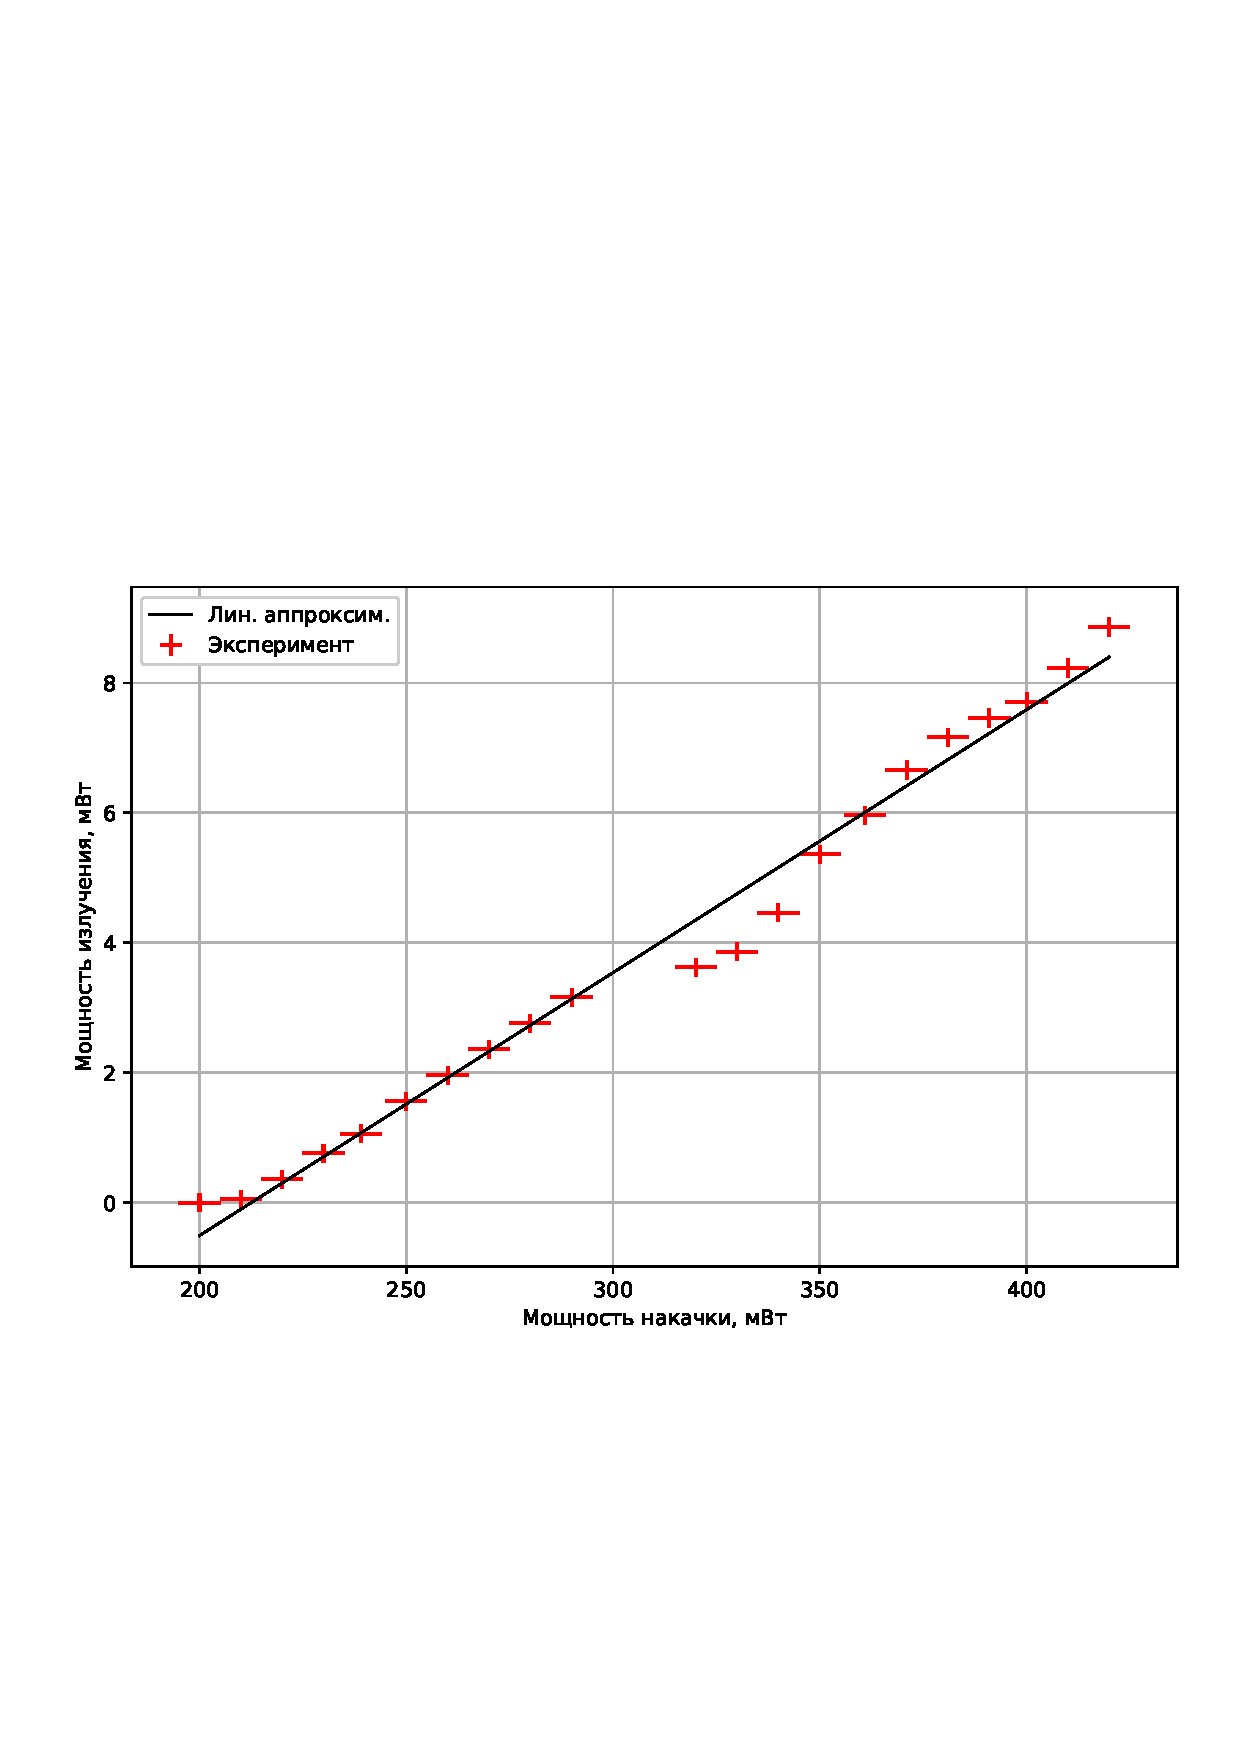
\includegraphics[width=\textwidth]{../figures/p_iz_vs_p_nak.png}
		\caption{Зависимость мощности излучения от мощности накачки. Фоновая засветка учтена и вычтена из мощности излучения.}
		\label{fig:p_iz_vs_p_nak}
	\end{figure}

	\subsection{Расчёт параметра G}

	



\end{document}